\documentclass[11pt, a4paper]{article}

\usepackage[utf8]{inputenc}
\usepackage[T1]{fontenc}
\usepackage[francais]{babel}
%\usepackage{xcolor}
\usepackage{amsmath}
\usepackage{amssymb}

\usepackage{amsthm}  %%%%% ajout 

%%%pour inclure des images
\usepackage{graphicx}
%TODO: \graphicspath{ {images/} }

\newtheorem*{theo}{Théorème (Rappel)} %%%%% ajout



\title{Résolution de l'équation de Laplace, par la méthode de Monte-Carlo}
\author{Victor \textsc{Schneider}, Christophe \textsc{Riviere}, Fabien \textsc{Delhomme}}
\begin{document}
%Définition de commandes
%\newcommand{\impo}[1]{\emph{#1}}
%Fin de définition de commandes
\maketitle
\begin{abstract}
    L'objectif de ce projet est de calculer une solution de l'équation de Laplace à l'aide de la
    méthode de Monte-Carlo.
\end{abstract}


\section{Présentation de la méthode de Monte-Carlo}

\subsection{Introduction}

La méthode de Monte-Carlo est une méthode d'approximation numérique qui s'appuie sur les propriétés
de la marche aléatoire.
\smallbreak
Cette méthode est très utilisée dans les domaines scientifiques nécessitant des approximations
numériques. Un exemple, lors de l'expérience permettant de mettre en évidence les oscillations des
neutrinos (en 2001), il était nécessaire de comparer les données énergétiques expérimentales avec
les valeurs numérique que donnait la théorie, valeurs qu'il a fallu estimer numériquement. On a
utilisé pour ce faire la méthode de Monte-Carlo.

%TODO changer la taille:
\begin{figure}
    \centering 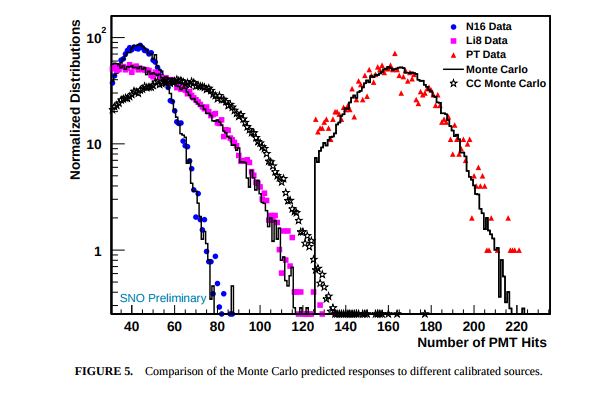
\includegraphics[width=10cm]{exMC}
    \caption{Exemple d'utilisation de la méthode de Monte-Carlo}
\end{figure}

source : http://arxiv.org/abs/nucl-ex/0110005v1 %TODO: mettre des liens dans les pdf

\subsection{Idée générale de la méthode}

\begin{theo}
    Théorème de transfert dans le cas d'une loi continue.

    Soit $f : \mathbb{R}^n \rightarrow \mathbb{R}$ la fonction densité associée à la variable
    aléatoire $X = (X_1, X_2,...,X_n)$.

    Alors\[
        \mathbb{E} \left( \phi(X_1, ..., X_n) \right) =  \int_{\mathbb{R}^n} \phi(x_1,...,x_n)f(x_1,...,x_n) \, \mathrm{d}x_1...\mathrm{d}x_n.
    \]
\end{theo}

Si l'on veut calculer une valeur numérique $A$ bien exprimée, on peut la voir grâce au théorème ci
-dessus comme une espérance. 

Soit $A$ notre valeur numérique à calculer sur un pavé,
\[
  A = \int_{[a,b]^n} \phi(x_1,...,x_n)f(x_1,...,x_n) \, \mathrm{d}x_1...\mathrm{d}x_n.
\]
Alors
\[
  A = \mathbb{E} \left( \phi(X_1, ..., X_n) \right).
\]
où les $X_i$ sont des variables indépendantes suivant toutes la loi uniforme sur $[a,b]$.
\medbreak
 L'idée derrière cette méthode est de pouvoir approximer une valeur numérique par une moyenne de
 marches aléatoires. Le théorème clef qui autorise cette démarche est la loi forte des grands
 nombres :

\begin{theo}
     Loi forte des grands nombres.

    Soit $(Y_k)_{k\ge 0}$ une suite de variables aléatoires indépendantes et suivant toutes la même
    loi, à valeurs dans $\mathbb{R}^n$. On suppose $\mathbb{E}(|Y_1|) < +\infty $. Alors

    \[
        \frac{Y_1+...+Y_N}{N}\underset{N\to+\infty}{\longrightarrow}\mathbb{E}(Y_1)\; \text{presque sûrement.}
    \]
\end{theo}

Autrement dit, si l'on prend un $N$ assez grand, on peut estimer une espérance de manière
relativement précise. On peut alors estimer notre valeur numérique $A$ "simplement" par une moyenne
de variable aléatoire. On peut donc utiliser cette méthode pour effectuer un calcul numérique de
$A$.

\[
    A \approx \frac{\phi(Y_1)+...+\phi(Y_N)}{N}
\]
où tous les $Y_i$ suivent la même loi que $X$ précédemment.

Or numériquement, on sait faire une moyenne, et on sait modéliser des variables aléatoires.



\subsection{Monte-Carlo appliquée à la résolution d'un problème de Laplace}

Nous allons nous utiliser cette méthode pour établir des solutions numériques à l'équation de Laplace en tout point du domaine.


\section{Schéma retenu}

\subsection{Discrétisation}
On commence par discrétiser le domaine choisi. On a choisi de quadriller le domaine.  Au début, nous
avons commencé par utiliser les coordonnées des points du plan puis exécuter la marche aléatoire en
«sautant» de points en points où la distance entre chaque saut est donnée par $1/N$, où $N$ était un
paramètre du schéma.  Malheureusement, au fur et à mesure des pas, à cause des erreurs d'arrondi, on
«sort» de la grille du domaine. Nous avons donc préféré construire une grille (une matrice) qui
représente les points du domaine, puis effectuer la marche aléatoire dans cette grille. Les indices
d'une matrice étant entier, il n'y a plus d'erreur d'arrondi possible.

La discrétisation s'effectue donc grâce à une matrice remplie de $1$ ou $0$ pour indiquer
respectivement si un point se trouve ou non dans le domaine.

\subsection{Marche aléatoire}

Il faut maintenant parcourir tout les points de la grille qui sont à l'intérieure du domaine.
Pour chaque point du domaine, on lance $K$  marches aléatoires qui commencent en ce point. On fait
ensuite la moyenne de toutes les valeurs données par la fonction au bord en tout les points à
l'extérieure du domaine atteint après une marche aléatoire.


\subsection{Paramètres du schéma}

\begin{itemize}
	\item $N$ correspond au nombres de carré de la grille qui discrétise le domaine. Plus ce nombre est
		élevé, plus la discrétisation est fine.
	\item $K$ nombre de marches aléatoires effectuées pour chaque points du plan.
\end{itemize}

\section{Convergence}

Pour analyser la convergence nous avons procédés comme il suit.

\section{Avantages et désavantages de la méthode de Monte-Carlo}

On voit tout de suite les intérêt de cette méthode pour le calcul de la solution de l'équation de
Laplace:
\begin{itemize}
	\item La relative simplicité du schéma: la seule difficulté qui s'est présentée fut de créer
		une grille pour lancer la marche aléatoire.
	\item Une parallélisation du calcul possible: la solution est construite point par point
		(!). En effet, contrairement aux schémas classiques qui calculent la valeur en
		chaque point en faisant la moyenne des points autour, ce schéma aléatoire peut par
		exemple calculer la solution en un point précis. On remarque aussi que l'on peut
		facilement stopper le calcul d'une solution pour le reprendre plus tard: il suffit
		de faire une moyenne des deux résultats.
\end{itemize}

On notera tout de même quelques désavantages:
\begin{itemize}
	\item Le bon fonctionnement de l'algorithme dépend en pratique d'un bon générateur de
		hasard. Ce sujet dépasse (de loin) le cadre de ce projet, mais il serait bon de
		vérifier la qualité du hasard proposée par \emph{Scilab}

	\item La difficulté théorique pour justifier la convergence du schéma: il nous faut en effet
		les résultats issue de la théorie de la probabilité, et en particulier de la marche
		aléatoire.
	% \item La convergence qui ne se fait que en $O(\sqrt{N})$. De plus, il est difficile de voir
	% 	comment améliorer cette convergence. Contrairement aux schémas classiques où il
	% 	suffit généralement d'un développement de Taylor à l'odre supérieure qui donne un
	% 	schéma qui converge plus vite (au prix de calcul plus compliqué certe).
\end{itemize}

\end{document}
